\documentclass{beamer}
%\documentclass{article}
%\usepackage{beamerarticle}
%\usepackage[french]{babel}
\usepackage[utf8]{inputenc}

\usepackage{graphicx}
\usepackage[english]{babel}
\usepackage{multimedia}


\usepackage{color}
\usepackage{graphicx}
\usepackage{alltt}
\usepackage{ulem}
\usepackage{amsmath} %bmatrix

\usepackage{tikz}
\usepackage{listings}

\usetheme{default}

\setbeamercolor{structure}{fg=black}
\setbeamercolor*{titlelike}{fg=black}

\setbeamertemplate{frametitle}
{\vskip1.6em
\insertframetitle\par
\vskip-1.6em
}
\setlength\parskip{0.1cm}

\newcommand\fullframegraphics[2]{
  {
    \setbeamertemplate{background}{\includegraphics[width=\paperwidth,height=\paperheight]{#2}}
    \begin{frame}
      \frametitle{#1}
    \end{frame}
  }
}

\lstset{%configuration de listings
language=C, 
float=hbp,% 
basicstyle=\ttfamily\scriptsize, % 
identifierstyle=\color{purple}, % 
keywordstyle=\color{red}, % 
stringstyle=\color{green}, % 
commentstyle=\color{gray}, % 
columns=flexible, % 
tabsize=2, % 
%frame=trBL, % 
%frameround=tttt, % 
extendedchars=true, % 
showspaces=false, % 
showstringspaces=false, % 
numbers=left, % 
numberstyle=\tiny, % 
breaklines=true, % 
breakautoindent=true, % 
captionpos=b,% 
xrightmargin=0cm, % 
xleftmargin=0cm 
}

\newcommand\showsaxpy[2]{\lstinputlisting[linerange=#1-#2,firstnumber=#1]{code/saxpy.c}}

%Junk to make nice agendas...
\makeatletter

\def\beamer@tableofcontents[#1]{
  \setcounter{tocdepth}{1}
  \begin{itemize}
    {\makeatletter \@input{\jobname.toc}}
  \end{itemize}
}

\def\beamer@sectionintoc#1#2#3#4#5{%
  {
    \ifnum\c@section>#1{
      \item \hyperlink{Navigation#3}{\planpast{#2}}
    }\else\ifnum\c@section=#1{
      \item \hyperlink{Navigation#3}{\plancurrent{#2}}
    }\else{
      \item \hyperlink{Navigation#3}{\planfuture{#2}}
    }\fi\fi
  }
}
\makeatother

%make a tableofcontents at the beginning of each section
\AtBeginSection[]{
  \frame<beamer>{\tableofcontents}
}

\setbeamertemplate{navigation symbols}{}%remove navigation symbols

\newcommand\planpast[1]{\textcolor{gray}{#1}}
\newcommand\plancurrent[1]{\textcolor{red}{#1}}
\newcommand\planfuture[1]{\textcolor{black}{#1}}

\newcommand\redbold[1]{\textcolor{red}{\bf #1}}

\setbeamertemplate{background}{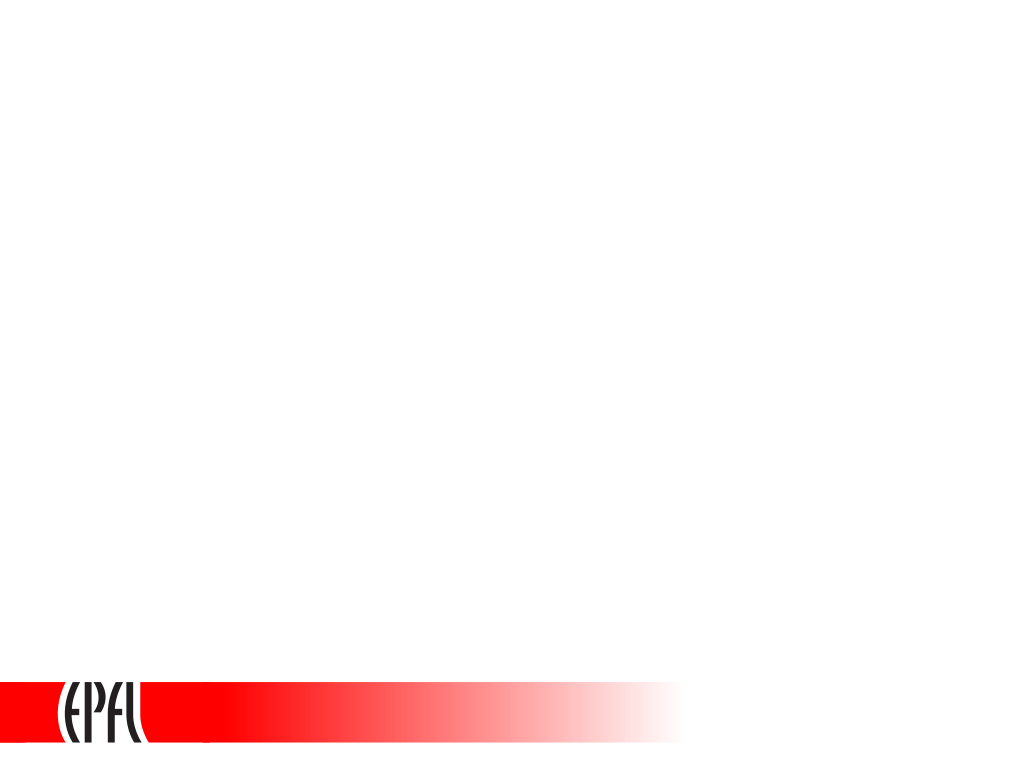
\includegraphics[width=\paperwidth]{images/wp.pdf}}
\setbeamercolor{structure}{fg=red}

\addtobeamertemplate{footnote}{}{\vspace{8ex}}

\title{Distributed network localization}
\author{Laurent Fasnacht, Matteo Pagliardini, Bernard Maccari}
\institute{Distributed Intelligent Systems}
\date{January 24, 2014}

\begin{document}

\begin{frame}
  \titlepage
\end{frame}

\section{Problem statement}
\section{Moore et al. approach}

\begin{frame}
    \frametitle{Flip ambiguity}
    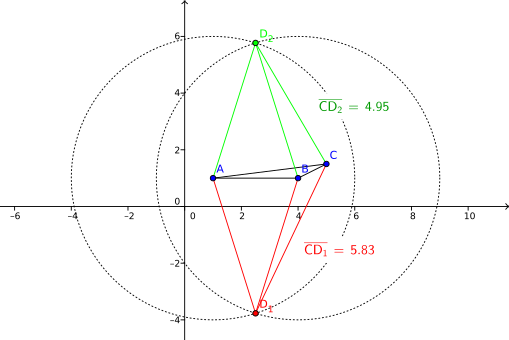
\includegraphics[width=\columnwidth]{schemas/FlipAmbiguity.pdf}
\end{frame}

\section{Our approach}
\begin{frame}
    \frametitle{Variance estimation}
    
    Use online algorithm (Donald Knuth, The Art of Computer Programming):
    
    Initialization: $n = 0$, $\mu = 0$, $M_2 = 0$ \\~
    
    New measurement $d$:
    \begin{itemize}
        \item $n \gets n+1$
        \item $\Delta \gets d - \mu$
        \item $\mu \gets \mu + \frac{\Delta}{n}$
        \item $M_2 \gets M_2 + \Delta \cdot (d-\mu)$
        \item $\sigma \gets \frac{1}{\mu}\sqrt{\frac{M_2}{n - 1}}$ (tend to \texttt{noise})
    \end{itemize}
\end{frame}

\begin{frame}
    \frametitle{New robust triangle criteria}
    \includegraphics{schemas/Gaussians.pdf}
    
    \begin{tabular}{ll}
        Original: &  $\min_{x,y \in T} d(x,y) \sin(\min_i \theta_i)^2 > k \sigma$ \\
        Our version: & $\sin(\min_i \theta_i)^2 > k \sigma$ \\
    \end{tabular}
\end{frame}

\begin{frame}
    \frametitle{Spring relaxation}
    \begin{center}
    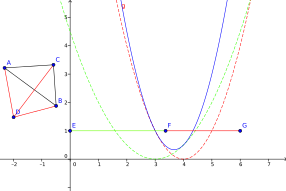
\includegraphics[width=0.7\columnwidth]{schemas/SpringRelaxation.pdf}
    \end{center}
    
    $F=-kx$, $P = 1/2 k x^2$
\end{frame}

\section{Results}
\section{Conclusion}
%\begin{frame}[fragile]
    %\lstinputlisting{code/intrinsics.c}
%\end{frame}


\end{document}
